This chapter will focus specifically on control rod cusping effects, which are the focus of this work.  First, a more thorough definition of the problem and motivation for solving it will be presented.  The next section will then present some of the solutions that have been used to minimize the cusping effects in the past, including a simplified decusping model implemented in MPACT itself.  The third section will then discuss some newer methods based on the sublpane CMFD scheme that have recently been implemented in MPACT.  Finally, a new ``sub-ray'' MOC method will be proposed to deal with the cause of the cusping effects on a more fundamental level.

\section{Background}

In Section \todo{section num}, some potential sources of errors for the 2D/1D scheme were introduced.  One of these was the error introduced by axial homogenization within a 2D MOC plane.  In some cases, this can be done without introducing significant errors.  For example, MPACT often homogenizes components outside the active fuel region, such as the end plugs and gaps at the end of the fuel rods.  However, when strong neutron absorbers, such as control rods, are homogenized axially in active fuel region, this has the effect of introducing absorption in regions where there should be none.  This effect is known as ``cusping,'' and is illustrated in Figure 

\begin{figure}
    \centering
    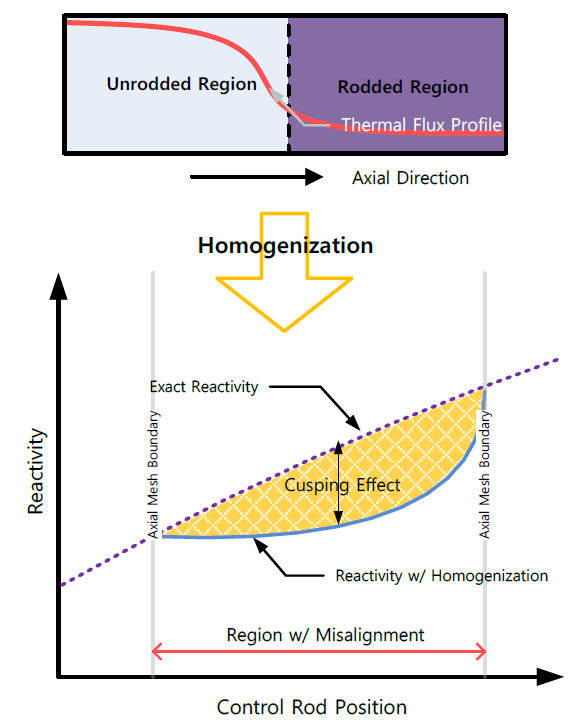
\includegraphics[width=0.4\textwidth]{figs/cusping_effect_Joo.png}
    \caption{Illustration of Rod ``Cusping''}\label{f:cuspingEffectJoo}
\end{figure}
\todo{cite}

In some cases, this is easily handled by setting up an appropriate axial mesh which prevents the need for the homogenization, but this is not always a practical solution.  Throughout the course of an entire cycle of operation (usually about 18 months), several different control banks in the reactor may move to a variety of positions to maintain criticality in the core.  Control rods in a PWR typically have step sizes of approximately 1.5 cm, but a typical MOC plane in MPACT is about 8 cm thick in the active fuel region.  In order to prevent cusping effects for an entire cycle, the user may have to create a very detailed axial mesh to ensure that all the control rod positions used throughout the cycle align with the edge of an MOC plane.  Not only is this tedious for the user, but it also greatly increases the computational burden due to the increased number of MOC planes.  Figure \ref{f:p4cuspingEffects} shows the calculated k-eff as a function of control rod position.  The cusping effects in this figure are further complicated by a heterogeneous rod with AIC and B$_4$C poison regions and a stainless steal tip.  Thus, cusping effects occur not just at the control rod tip, but also at material interfaces throughout the rod.

\begin{figure}
    \centering
    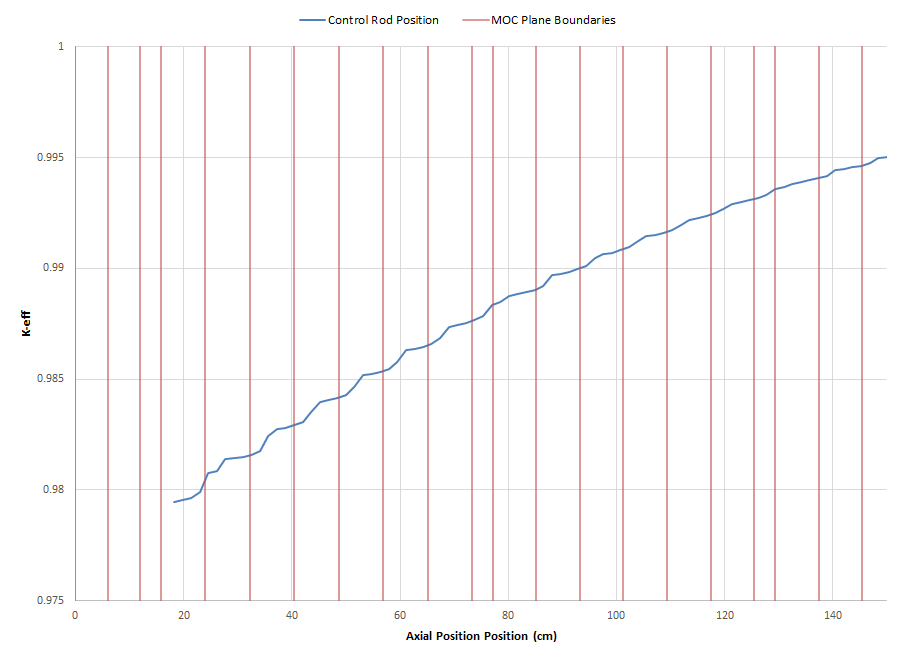
\includegraphics[width=0.8\textwidth]{figs/p4cuspingEffects.png}
    \caption{Control Rod Cusping Effects for 3x3 Assembly}\label{f:p4cuspingEffects}
\end{figure}

\section{Traditional Solutions}

\subsection{Nodal Codes}

\hl{Discuss ways people have addressed this in the past}

\subsection{2D/1D Codes}

Several codes that have employed the 2D/1D method in recent years have also required rod decusping methods.  MPACT currently uses a simple polynomial correction to the volume fractions used to homogenize the control rod \cite{MC2015_VCS_Cycle_Depletion}.  To develop this method, a 3x3 assembly was set up with a control rod in the center assembly.  This problem was simulated with the rod tip at nine different positions in the plane.  These simulations were then repeated, but with the axial mesh refined so the rod tip aligned with a plane boundary.  The k-eff differences between the two sets of simulations were fitted with a sixth-order polynomial which is used in MPACT to reduce the volume fraction of the control rod by an appropriate amount to offset the cusping effects.  This process was repeated for different control rod materials such as AIC, B$_4$C, and Tungsten, since each material has unique cross-sections.  This method has the advantages of being simple to implement and requiring no increase in computational requirements.  However, the results obtained from this decusping method are tied to the control rod material and reactor model used to develop the corrections, limiting its usefulness to a small subset of reactors.

Another 2D/1D code is nTRACER, which is under active development by \hl{some people in Korea}.  To address rod cusping effects in nTRACER, \hl{Korean guy}, et al. developed a more general method than the polynomial correction method used by MPACT\todo{cite ICAPPS}.  This method pre-generates correction factors at the start of a simulation, rather than relying on hard-coded corrections.  To do this, the assembly that will have a partially inserted control rod is identified, and a single-plane 3x3 assembly problem is set up using the partially-rodded assembly and its neighbors.  The radial and axial cusping effects are then determined separately.  First, the radial cusping effects are determined by performing 2D MOC calculations on the 3x3 sub-domain with the rod fully inserted and fully withdrawn.  This provides radial flux profiles in the rodded assembly for both rodded and unrodded regions, as well as current coupling coefficients for CMFD for the rodded and unrodded CMFD nodes.  Once this is done, the rod is simulated at positions of 25\%, 50\%, and 75\% withdrawn from the plane.  To reduce runtime, these calculations are done using only 3D sub-plane CMFD.  This generates axial flux profiles for the full MOC plane for each of the possible rod positions.  During the full-core 2D/1D calculation, these axial flux profiles are then used to generate improved homogenized cross-sections for the MOC calculation using equation \cite{ICAPPcontrolRodDecuspingNTRACER}.

\begin{equation}\label{e:nTRACERdecusping}
\overline{\Sigma_i} = \frac{\phi_{rad,i}^R \phi_{ax,i}^R \Sigma_i^R h^R + \phi_{rad,i}^U \phi_{ax,i}^U \Sigma_i^U h^U}{\phi_{rad,i}^R \phi_{ax,i}^R h^R + \phi_{rad,i}^U \phi_{ax,i}^U h^U}
\end{equation}

\hl{DeCART?  Other 2D/1D codes?}

\section{Improved Decusping Methods}
\todo{Better Title?  Not that much ``better''}

This section discusses two new decusping treatments added to MPACT.  These methods rely on the sub-plane scheme described in section \todo{ref}.  The first method only treats the axial cusping effects, while the second method extends the first by also treating the radial decusping effects.

\subsection{Sub-plane Decusping}

In section \todo{section num}, the sub-plane scheme was introduced as a means of coarsening the 2D/1D axial mesh to improve runtime while maintaining accuracy.  However, one negative consequence of using the sub-plane scheme is that it increases the likelihood of partially inserted rods being present since there are fewer, thicker MOC planes.  To address this, two modifications were made to the sub-plane scheme to minimize cusping effects.

The first modification that was made was to modify the cross-sections used for the sub-plane CMFD and axial SP$_3$ calculations.  In the most basic form of the sub-plane scheme, the same cross-sections and radial coupling coefficients are used for all sub-planes in each MOC plane.  To use sub-plane as a decusping method, the requirement for constant cross-sections was removed.  Thus, when equation \ref{e:CMFDhomogTerms} is applied, explicit rodded or unrodded cross-sections are used for the cross-section homogenization in each sub-plane, rather than a single homogenized cross-section being using in all sub-planes.  This allows the CMFD and axial solvers to capture the sharp flux gradients that occur around the edge of the control rods.

\hl{Radial coupling coefficients still axially flat for each MOC plane}

In order to improve the MOC calculations as well, the CMFD flux projection described in equation \ref{e:CMFDscaling} is extended to also include a cross-section projection for the partially rodded pin cells.  This is done using equation \ref{e:nTRACERdecusping} with $\phi_{rad,i}^R = \phi_{rad,i}^U$.  This allows the 2D MOC calculations to also capture some of the axial effects of the partially inserted rod.

\todo{Runtime results here? 2D/1D section? Anywhere?}

%\begin{table}
%\caption{Comparison of MPACT and DeCART subplane scheme results for C5G7-like rodded problem}
%\begin{center}
%\begin{tabular}{|l|c|c|c|c|c|c|}\hline
%Plane & \multicolumn{2}{|c|}{k-eff Diff.} & \multicolumn{2}{|c|}{Max Power Diff.} & \multicolumn{2}{|c|}{Relative Runtime} \\ \cline{2-7}
%Division & MPACT & DeCART & MPACT & DeCART & MPACT & DeCART \\ \hline
%2 & 0.6 & 5.2 & 0.003\% & 0.04\% & 0.579 & 0.513 \\ \hline
%3 & 1.9 & 7.7 & 0.004\% & 0.10\% & 0.408 & 0.327 \\ \hline
%5 & 2.2 & 9.5 & 0.008\% & 0.11\% & 0.350 & 0.214 \\ \hline
%10 & 1.2 & 9.8 & 0.020\% & 0.22\% & 0.253 & 0.058 \\ \hline
%\end{tabular}
%\end{center}
%\end{table}
%
%\begin{table}
%\caption{Comparison of subplane scheme to traditional 2D/1D for VERA Progression Problem 4}
%\begin{center}
%\resizebox{\textwidth}{!}{\begin{tabular}{|l|c|c|c|c|c|c|c|c|}\hline
%Number & k-eff Diff. & \multicolumn{2}{|c|}{Power Diff.} & \multicolumn{2}{|c|}{Outer Iterations} & \multicolumn{3}{|c|}{Runtime (core-hours)} \\\hline
%of Planes & (pcm) & RMS & Max & Traditional & Subplane & Traditional & Subplane & Ratio ($\frac{Subplane}{Traditional}$) \\\cline{3-9}
%32 & 0.01 & 0.001\% & 0.004\% & 29 & 30 & 21.0 & 16.2 & 0.77 \\\hline
%46 & 0.01 & 0.018\% & 0.053\% & 14 & 21 & 10.3 & 8.9 & 0.86 \\\hline
%62 & 0.04 & 0.023\% & 0.056\% & 12 & 20 & 12.4 & 11.5 & 0.93 \\\hline
%77 & 0.04 & 0.022\% & 0.067\% & 12 & 21 & 13.0 & 11.4 & 0.88 \\\hline
%\end{tabular}}
%\end{center}
%\end{table}
%
%\begin{table}
%\caption{Comparison of subplane scheme to traditional 2D/1D for VERA Progression Problem 5}
%\begin{center}
%\resizebox{\textwidth}{!}{\begin{tabular}{|l|c|c|c|c|c|c|c|c|}\hline
%Number & k-eff Diff. & \multicolumn{2}{|c|}{Power Diff.} & \multicolumn{2}{|c|}{Outer Iterations} & \multicolumn{3}{|c|}{Runtime (core-hours)} \\\hline
%of Planes & (pcm) & RMS & Max & Traditional & Subplane & Traditional & Subplane & Ratio ($\frac{Subplane}{Traditional}$) \\\cline{3-9}
%32 & 0.01 & 0.004\% & 0.008\% & 28 & 29 & 996  & 1325 & 1.33 \\\hline
%46 & 0.11 & 0.044\% & 0.111\% & 13 & 29 & 691  & 829  & 1.20 \\\hline
%62 & 0.07 & 0.028\% & 0.190\% & 12 & 46 & 880  & 918  & 1.04 \\\hline
%77 & 0.08 & 0.030\% & 0.184\% & 12 & 45 & 1090 & 1013 & 0.93 \\\hline
%\end{tabular}}
%\end{center}
%\end{table}

\subsection{Auxiliary 1D Collision Probabilities}

While the sub-plane decusping method is better than none, it captures only the axial effects of the partially inserted rod.  To also capture the radial effects, an additional radial calculation is needed to obtain radial flux profiles for the rodded and un-rodded regions.  In MPACT, this is done using a 1D Collision Probabilities (CP) solver.

After the CMFD homogenization, but prior to the calculation itself, a 1D CP kernel is solved for the rodded and un-rodded regions to obtain a radial flux profile.  These profiles are normalized so that the volume-average of each profile is exactly unity.  These profiles are then used with the sub-plane CMFD flux and material cross-sections to calculate improved homogenized cross-sections, as shown in equation \ref{e:CPMxs}.  Homogenizing the cross-sections in this way allows CMFD to capture both axial and radial effects of the partially inserted rod with negligible increase in computational expense.  This process is illustrated in figure \ref{f:CPdecusp}.

\begin{equation}\label{e:CPMxs}
\Sigma_{g,i}=\frac{1}{\phi_{g,i}V_i}\sum_{r=1}^{N_{rings}} \Sigma_{g,r} \phi_{CMFD,g,i} \phi_{CP,g,r} V_r
\end{equation}

\begin{figure}
  \centering
  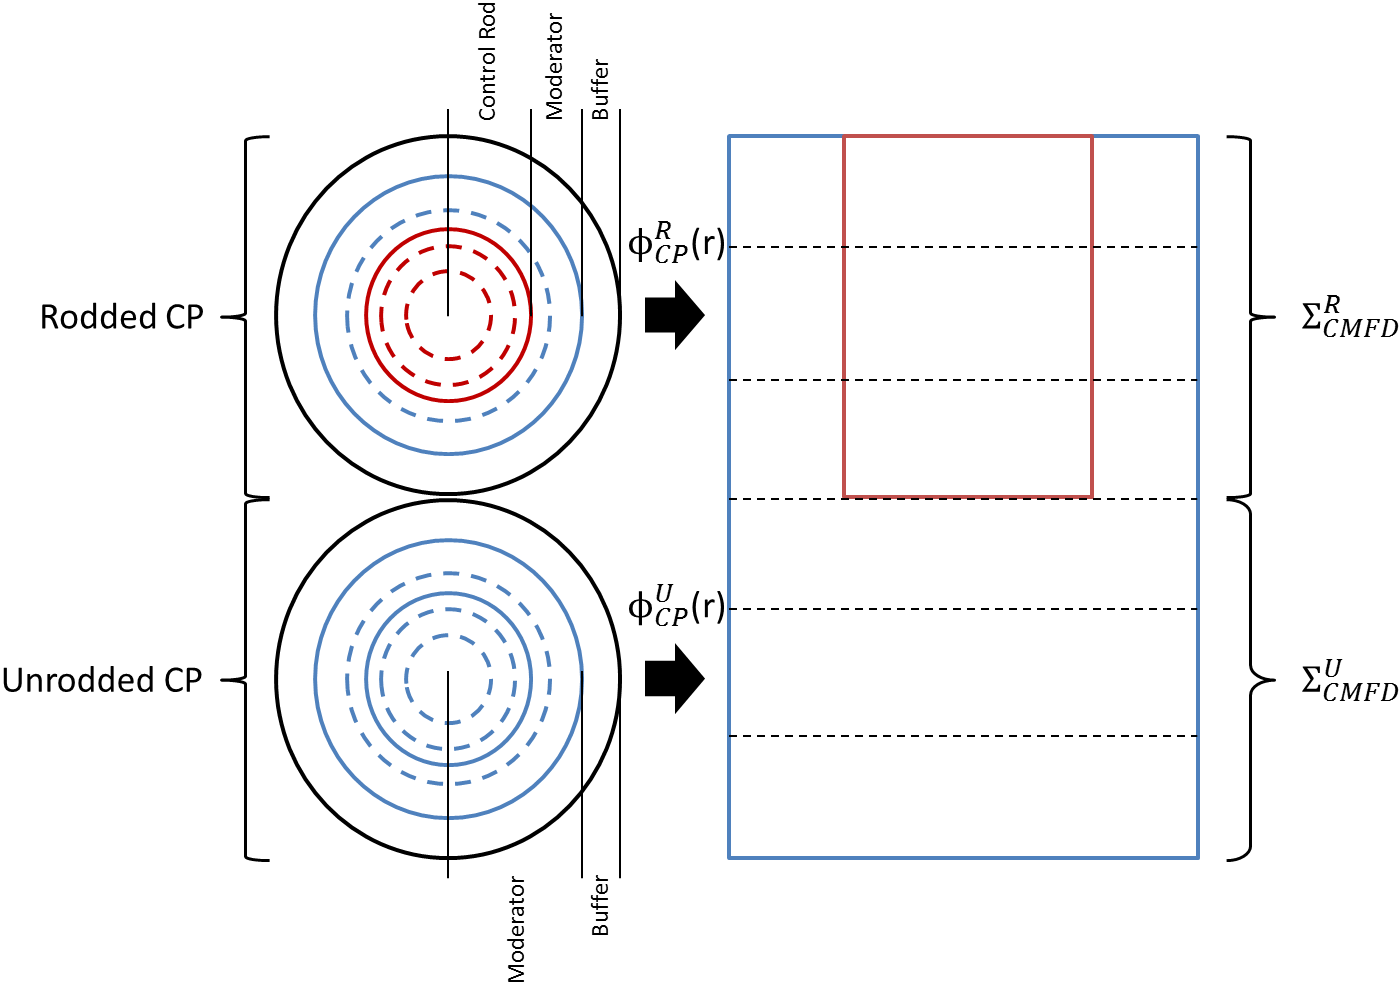
\includegraphics[width=\textwidth]{figs/CPdecusp.png}
  \caption[Collision Probabilities Decusping]{Illustration of 1D Collision Probabilities rod decusping method}\label{f:CPdecusp}
\end{figure}

After the CMFD calculation, the MOC cross-sections must be modified as with the sub-plane decusping.  This is done using by using equation \ref{e:nTRACERdecusping} directly, where the radial flux terms are the projected MOC fluxes and the axial flux terms are the results of the sub-plane CMFD calculation that used the CP-homogenized cross-sections.  The projection of the CMFD flux to the MOC mesh is unchanged from the standard sub-plane scheme.  The CMFD calculation flow when using 1D CP is shown in figure \ref{f:1dcpm-flowchart}

\begin{figure}
  \centering
  \begin{tikzpicture}[node distance=2cm]

% Start
\node (start) [startstop] {Start};

% CMFD
\node (homog) [process, right of=start, xshift=2.0cm] {Homogenize cross-sections and flux; Calculate $\tilde{D}$};
\node (1dcpm) [process, below of=start, yshift=-0.5cm] {1D CP calculations};
\node (homogCP) [process, right of=1dcpm, xshift=2.0cm] {Re-homogenize cross-sections in partially rodded pin cells};
\node (iterCheck) [decision, below of=homogCP, yshift=-1.5cm] {First iteration?};
\node (firstIter) [process, below of=iterCheck, xshift=-2.5cm, yshift=-1.0cm] {Set $\hat{D}=0$};
\node (laterIter) [process, below of=iterCheck, xshift=2.5cm, yshift=-1.0cm] {Calculate $\hat{D}$};
\node (matrix) [process, below of=firstIter, xshift=2.5cm] {Set up CMFD matrix};
\node (3DCMFD) [process, below of=matrix] {3D CMFD calculation};
\node (proj) [process, below of=3DCMFD] {Scale MOC flux with CMFD flux};
\node (projCP) [process, below of=proj] {Homogenize partially rodded MOC cross-sections};

% Stop
\node (stop) [startstop, right of=projCP, xshift=2.0cm] {Stop};

% Basic Arrows
\draw [arrow] (start) -- (homog);
\draw [arrow] (1dcpm) -- (homogCP);
\draw [arrow] (homogCP) -- (iterCheck);
\draw [arrow] (matrix) -- (3DCMFD);
\draw [arrow] (3DCMFD) -- (proj);
\draw [arrow] (proj) -- (projCP);
\draw [arrow] (projCP) -- (stop);

% Fancy Arrows
\draw [arrow] (homog) |- ([yshift=-0.75cm]start.south) -| (1dcpm);
\draw [arrow] (iterCheck) -| node[anchor=south] {yes} (firstIter);
\draw [arrow] (iterCheck) -| node[anchor=south] {no} (laterIter);
\draw [arrow] (firstIter) |- (matrix);
\draw [arrow] (laterIter) |- (matrix);

\end{tikzpicture}
  \caption[Stuff]{Calculation flow for CMFD calculation in MPACT with 1D CP decusping treatment}\label{f:1dcpm-flowchart}
\end{figure}

\section{Future Work}

Moving forward, there are several improvements that can be made to the 2D/1D scheme with regard to the cusping problem.  Four of these improvements will be discussed in this section.  The first two are modifications to methods already in MPACT, while the second two would involve implementation of new solvers.

\subsection{Axial Transverse Leakage Source}

The first improvement that could be made is in the axial transverse leakage source.  As discussed in section \todo{number}, the axial TL is calculated on the homogenized CMFD mesh by the axial solver (usually SP$_3$).  Because of this, it is assumed to be spatially flat within each pin cell.  However, the energy dependence of the flux and current are completely different between the fuel and moderator.  This is also true for a rodded pin cell due to the control rod being a strong absorber.  Thus, the results of the MOC calculations could be improved by treating the spatial dependence of the axial TL source within each pin cell.  \todo{prior work?}

\subsection{Radial Transverse Leakage Source}

A second improvement that could be made is to improve the resolution of the radial TL source when using the sub-plane--based decusping methods.  The current implementation assumes the same $\hat{D}$ current correction term for all sub-plane surfaces between two pin cells.  This assumption is made to improve the stability of the sub-plane scheme, but certainly introduces some error in the CMFD and SP$_3$ calculations.  When a control rod is partially inserted into an MOC plane, this error is greater than normal since the currents in the rodded sub-planes should be much different from those in the unrodded sub-planes.  Introducing a better shape to the $\hat{D}$ terms would certainly improve the overall accuracy of the calculations.

\subsection{Auxiliary Solver}

Another potential source of error for the decusping treatments discussed here is in the choice of auxiliary solver.  The 1D CP kernel was useful for capturing some of the radial cusping effects, but it does have some deficiencies.  First, because it is 1D, it ignores the corner effects of the pin cell by treating the moderator as a ring.  This minimizes the directional dependence of the neutrons, changing the radial flux profile generated by the solver.  Second, the 1D CP solver relies on a buffer region obtained by homogenizing the surrounding pin cells.  As with the moderator region, this buffer region is assumed to be annular and homogeneous.  This affects the source term which drives the problem and the behavior of the neutrons which escape the pin cell of interest.

One way to address this would be to use a highly optimized MOC solver.  Solving only a single pin cell with MOC would have minimal impacts on runtime, but would successfully capture the corner effects and more accurately handle the boundary conditions by directly using the results of the full-plane 2D MOC calculations.  This method should show some improvement over the 1D CP method that is currently used.

\subsection{Sub-Ray MOC}

The final potential improvement that will be discussed here is a new ``sub-ray'' MOC method.  This method is still being developed, but will be tested in MPACT to continue this work.  Sub-ray MOC will be treated like regular 2D MOC in most of the 2D plane.  As a ray is swept, the outgoing angular flux and scalar flux contribution for each region is calculated, along with currents at the pin cell boundaries.  However, upon entering a partially rodded region, the ray will ``split.''  The calculations will be done twice in that region: once using a rodded cross-section and source, then a second time using an unrodded cross-section and source.  This will continue until the rodded and unrodded angular fluxes have converged toward each other, at which point the sub-rays will end and become a single MOC ray again.

This method has a significant advantage over other decusping methods because it directly calculates an improved angular flux, which is the fundamental quantity from which other MPACT results are calculated.  If the angular flux is correct, then all other quantities such as scalar flux, current, and power will be correct as well.  Furthermore, this method could prove to be useful for components besides control rods.  For example, spacer grids, burnable poison inserts, and axial blankets are just three examples of reactor components which usually require additional MOC planes in the 2D/1D method.  However, if sub-ray MOC is used, it should negate the requirement for additional MOC planes, further reducing the computational burden of the calculations.

Several questions must be worked out for the sub-ray MOC method.  The first concerns how to combine the sub-ray angular fluxes.  It is possible that calculating the angular fluxes for each axial level explicitly will allow them to be mixed using the rodded and unrodded volume fractions, but something more advanced may be required.  Additionally, it is not known yet how long the sub-rays must exist before recombining to a single ray.  Each of these questions is discussed in further detail in section \todo{num}, where some results from a 1D MOC code are presented.